\documentclass[12pt]{article}
\usepackage{graphicx}
\def\baselinestretch{3.0}
\setlength{\topmargin}{0pt}
\setlength{\textheight}{570pt}
\setlength{\oddsidemargin}{0pt}
\setlength{\evensidemargin}{60pt}
\setlength{\textwidth}{427pt}
%\setlength{\footheight}{0pt}
%\setlength{\footskip}{30pt}
\parindent 15pt
\hyphenpenalty=10000
\tolerance=10000
\pagestyle{empty}
\def\ul{\underline}
\def\fn{\footnotemark\ }

\begin{document}

\centerline{\bf Inferring Phylogenies from Protein Sequences by}
\bigskip

\centerline{\bf Parsimony, Distance, and Likelihood Methods}
\vfill

\centerline{Joseph Felsenstein}
\vfill

\begin{center}
Department of Genetics\\
University of Washington\\
Box 357360\\
Seattle, Washington 98195-7360\\
USA\\
~\\
E-mail: joe@genetics.washington.edu
\end{center}
\vfill
(Send proofs to me at above address)
\vfill


\centerline{Running Head: Phylogenies from Protein Sequences}
\vfill

\newpage
\pagenumbering{arabic}
\pagestyle{headings}

The first molecular sequences available were protein sequences, so it is not
surprising that the first papers on inferring phylogenies from molecular
sequences described methods designed for proteins.  Eck and Dayhoff\fn
described the first molecular parsimony method, with amino acids as the
character
states.  Fitch and Margoliash\fn initiated distance matrix phylogeny
methods with analysis of cytochrome sequences.  Neyman\fn  presented the
first likelihood method for molecular sequences, using a model of symmetric
change among all amino acids.

After a long period in which attention shifted to nucleotide sequences,
attention is again being paid to models in which the amino acid sequences
explicitly appear.  This is not only because of the increased availability
of protein sequence data, but because the conservation of amino acid
sequence and protein structure allows us
to bring more information to bear on ancient origins of lineages and of genes.

I will here briefly review the work on using protein sequence and structure to
infer phylogeny, in the process describing some methods of my own.

\section* {Parsimony}

Eck and Dayhoff's paper\footnotemark[1]\ did not describe their algorithms in enough
detail to reproduce them, but it is apparent that the model of amino acid
sequence evolution they used did not take the genetic code into account.  It
simply considered the amino acids as 20 states, with any change of state able
to result in any of the other 19 amino acids.  The realization that more
information could be extracted by explicitly considering the code shortly led
to more complex models.  Fitch and Farris\fn gave an approximate
algorithm to calculate for any set of amino acid sequences, on a given tree,
how many nucleotide substitutions must, at a minimum, have occurred.  As
certain amino acid replacements would then require 2 or 3 base substitutions,
this would differentially weight amino acid replacements.  Moore\footnotemark$^,$\fn
had already presented an exact, though more
tedious, algorithm to count the minimum number of nucleotide substitutions
needed, and he pointed out the approximate nature of Fitch and Farris's
method\footnotemark.

These papers might have settled the matter for the parsimony criterion, except
that they count as equally serious those nucleotide substitutions that do and
do not change the amino acid.  For example, we might have a Phenylalanine
that is coded for by a UUU, which ultimately becomes a Glutamine that is coded for by
a CAA.  This requires three nuclotide substitutions.  It is possible for
one of these to be silent, as we can go from UUU (Phe) $\rightarrow$ CUU (Leu)
 $\rightarrow$ CUA (Leu) $\rightarrow$ CAA (Glu).  Presumably the second
of these changes will not be as improbable as the others, as it will not have
to occur in the face of natural selection against change in the amino
acid, or wait for a change of environment or genetic background that
favors the amino acid replacement.

In the PROTPARS program of my PHYLIP package of phylogeny programs, I have
introduced (in 1983) a parsimony method that attempts to reflect
this.  In the above sequence
it counts only two changes, allowing the silent substitutions to take place
without penalty.  In effect the method uses the genetic code to designate which
pairs of amino acids are adjacent, and allows change only among adjacent
states.  Sankoff\fn and Sankoff and Rosseau\fn have presented a
generalized parsimony algorithm that allows us to count on a given tree
topology how many changes of state are necessary, where we can use an arbitrary
matrix of penalties for changes from one state to another.  
The PROTPARS algorithm is equivalent to Sankoff's algorithm, being quicker but
less general. 

The set of possible amino acid states in the PROTPARS algorithm has 23 members,
these being the 20 amino acids plus the possibilities of a gap and a stop codon.
Serine is counted not as one amino acid but as two, corresponding to the
two ``islands" of serine codons in the genetic code.  These are
\{UCA, UCG, UCC, UCU\} and \{AGU, AGC\}, which make serine the only amino acid
whose codons fall into two groups that cannot be reached from each other by
a single mutation.  PROTPARS copes with this by regarding them as two amino acid
states (ser1 and ser2) and treats an observation of ``serine" as an ambiguity between
these two.

Imagine that we know, for a node in the tree, the set of amino acid states
that are possible at this node.  If the node is a terminal (tip) species,
these are just the observed amino acid, there being more than one if serine
is observed or if any of asn, gln, or glx are observed.  There is also the
possibility that the amino acid is unknown, but known not to be a gap, and
the possibility that the amino acid could be any one including a gap.  More
complex ambiguities are also possible and can arise in the process of reconstruction
of the states at interior nodes in the tree.  Any of these can be represented
by designating the members of the set $\ul{S}_{\ul{0}}$ of possible states.

Given the particular version of the genetic code that we are using, we can
also precompute, for each amino acid $\ul{a}$, the set $\ul{N}_{\ul{a}}$ of amino acid states that are one or
fewer steps away.  In PROTPARS, gaps are counted as being 3 steps away from
all the amino acids and from stop codons.  Having these precomputed sets allows
us to take the sets
$\ul{S}_{\ul{0}}$ at the tips of the tree, and compute for them $\ul{S}_{\ul{1}}$ and $\ul{S}_{\ul{2}}$, the sets
of amino acid states 1 or fewer steps away, and 2 or fewer steps away.  In
our program, all states, including gaps, are 3 or fewer steps away, so that
we do not need a set $\ul{S}_{\ul{3}}$.  In PROTPARS
the three sets $\ul{S}_{\ul{0}}$, $\ul{S}_{\ul{1}}$, and $\ul{S}_{\ul{2}}$ are updated down the tree, and the
number of steps needed for the tree counted, in the following way.

Imagine that there is an internal node in the tree with two descendants,
and whose sets of possible states are the $\ul{L}_{\ul{i}}$ and the $\ul{R}_{\ul{i}}$.
We are computing the sets $\ul{S}_{\ul{i}}$ for the internal node.  First, $\ul{L}_{\ul{0}}$ and $\ul{R}_{\ul{0}}$ are
compared.  If they are the same then the $\ul{L}_{\ul{i}}$ must be identical to the $\ul{R}_{\ul{i}}$,
and the $\ul{S}_{\ul{i}}$ are simply set to be the $\ul{L}_{\ul{i}}$, and no steps are counted.
Otherwise, we compute the four sets
\begin{equation}
\begin{array}{c c l}
T_0 & = & L_0 \cap R_0\\
T_1 & = &(L_1 \cap R_0) \cup (L_0 \cap R_1),\\
T_2 & = &(L_2 \cap R_0) \cup (L_1 \cap R_1)\cup (L_0 \cap R_2),\\
T_3 & = &R_0 \cup (L_2 \cap R_1) \cup (L_1 \cap R_2) \cup L_0.
\end{array}
\end{equation}
\noindent
They are
computed one after the other.
Their interpetation is straightforward.  For example, $\ul{T}_{\ul{1}}$ is the set of
amino acid states that, if present at the internal node, requires one
step to give rise to $\ul{L}_{\ul{0}}$ and none to give rise to $\ul{R}_{\ul{0}}$, or else
one step to give rise to $\ul{R}_{\ul{0}}$ and none to give rise to $\ul{L}_{\ul{0}}$.  Thus it
is the set of states which, if present at the interior node, require one
extra step in the subtree that is above that node.
As soon as one of these, say $\ul{T}_{\ul{k}}$, turns out to be nonempty, we know that
a minimum of $\ul{k}$ more steps will be needed at this node, and that the set $\ul{S}_{\ul{0}}$ for that node will be
$\ul{T}_{\ul{k}}$.   $\ul{T}_{\ul{3}}$ at least must be nonempty, as it contains the union of
$\ul{R}_{\ul{0}}$ and $\ul{L}_{\ul{0}}$.

Now, having found $\ul{S}_{\ul{0}}$, all we need to do is to compute $\ul{S}_{\ul{1}}$ and $\ul{S}_{\ul{2}}$ for the internal node.  The formulas
for doing so are
\begin{equation}
S_k = \bigcup_{a \in S_{k-1}} N_a, \qquad k = 1, 2
\end{equation}
This of course does not need to be done if $\ul{L}_{\ul{0}} = \ul{R}_{\ul{0}}$, as the sets $\ul{L}_{\ul{1}}$
and $\ul{L}_{\ul{2}}$ (or $\ul{R}_{\ul{1}}$ and $\ul{R}_{\ul{2}}$) can then be used directly.
   
This method of calculation using sets is equivalent to having a vector of
numbers, one for each amino acid state, which are 0, 1, 2, or 3.
The Sankoff
algorithm asks us to specify for each state the number of extra steps that
would be required above that point in the tree if that state existed in
that internal node.  In our model the possible values for the number of
extra steps are 0, 1, 2, and 3.  The sets
$\ul{S}_{\ul{i}}$ are just the amino acids which would have the number of extra steps less than or equal to $\ul{i}$.
The algorithm is then equivalent to the appropriate application of the
Sankoff algorithm.  It could probably be speeded up further, as most of the
time the set $\ul{S}_{\ul{2}}$ is the set of all amino acids, and that could be used as
the basis for some further economies.

Figure 1 shows the sets that would be stored on a small sample tree for
one amino acid position, and the counting of steps.  At each node the three
sets $\ul{S}_{\ul{0}}$, $\ul{S}_{\ul{1}}$, and $\ul{S}_{\ul{2}}$ are shown, and at interior nodes the number of
steps that are counted are also shown in circles.  There are 4 different
amino acids at the tips of the tree.  If any amino acid could change to any
other the tree would require only 3 steps, but in my protein parsimony model it
requires 5.

Protein parsimony methods exactly equivalent to PROTPARS are also available in
the programs PAUP and MacClade, using predefined matrices of costs of subtitution between
amino acid states, with the costs being taken into account by the Sankoff
algorithm.

\section*{Distances}

Distance-matrix methods calculate for every pair of sequences an estimate of
the branch length separating them, where branch length is the product of
time and rate of evolution.  That tree is then chosen that, by some criterion,
makes the best prediction of these pairwise distances.  For protein sequences
we need to specify a probabilistic model of evolution.  Jukes and Cantor\fn
were the
first to do this for protein sequences (see also Farris\footnotemark).  This model was highly oversimplified,
as it had equal probabilities of change between all pairs of amino acids.
Dayhoff and Eck\footnotemark and Dayhoff \ul{et. al.}\fn empirically tabulated probabilities of change between amino
acids over short evolutionary times, producing a table of transition
probabilities between amino acids.  This model does not take explicit account
of the genetic code, and is subject to errors from the limited sample size
on which it was based.  Nevertheless the genetic code should affect its
transition probabilities, and so should the biochemical properties of the
amino acids.  A more recent empirical model of amino acid change is that of
Jones \ul{et. al.}\footnotemark.  They have also produced models for specific subclasses
of proteins, that may be more useful in those contexts\footnotemark.
Other recent compilations of scoring matrices for evaluating the similarity
of amino acid sequences\footnotemark$^,$\fn are not in the form of transition probability tables.
For this reason they cannot be used to compute the branch length estimates that
we require here.

A naive alternative to these empirical matrices is to divide the amino
acids into a number of categories, based on their chemical properties.
Suppose that we imagine mutations occurring in the genetic code table, with
the starting points being codons generated at random from a given base
composition.  Now imagine single base substitutions.  If these do not
change the biochemical class of the amino acid, they are accepted; if they
do, they are only accepted with probability $\ul{p}$.  We omit the stop codons
from consideration: if either the starting point or the destination of a
change is a stop codon, the change is not made.  This model, once given the
amino acid categories,
the base frequencies and the probability $\ul{p}$, generates a transition probability
table between all pairs of amino acids.

Version 3.5 of PHYLIP contains a program, PROTDIST, which computes distances
based either on the PAM001 model\footnotemark[13]\  and the transition probability matrix
generated by the categories model.  It also can
compute distances using the formula of Kimura\fn which bases the distance
on the fraction of amino acids shared between the sequences, without regard to
which amino acids they are.  The categories model, as implemented in PROTDIST,
can use several different genetic codes (the universal code and several kinds
of mitochondrial code).  Three categorizations of the amino acids are used,
one the categories given by George \ul{et. al.}\fn, one from a categorization
in a ``baby biochemistry" text, and one the opinion of a colleague.  Interestingly, all three of these turn out to be subdivisions of one linear order of amino
acids.  We have
found that a value of $\ul{p} = 0.45$ brings the ratio of between- to within-category
change in the category model of George \ul{et. al.}\footnotemark[19] close to that in the Dayhoff model.  In the next release (4.0) of
PHYLIP, we hope to expand the range of models by including the 
model of Jones \ul{et. al.}\footnotemark[14], and allowing for a Gamma distribution of evolutionary rates among
sites, in the manner of Jin and Nei\fn and Nei \ul{et. al.}\footnotemark.

Given the evolutionary model, we use maximum likelihood estimation to
compute the distances.  In effect we are specifying a two-species tree, with
but one branch, between the pair of species, and estimating that branch length
by maximum likelihood.  If we observe $\ul{n}_{\ul{ij}}$ changes between amino acids
$\ul{i}$ and $\ul{j}$, and if the model we are using has equilibrium frequency $\ul{f}_{\ul{i}}$ for
amino acid $\ul{i}$ and transition probability $\ul{P}_{\ul{ij}}(\ul{t})$ over time $\ul{t}$,
the expected fraction of sites which will have amino acid $\ul{i}$ in one species
and $\ul{j}$ in the other is $\ul{f}_{\ul{i}} \ul{P}_{\ul{ij}}(\ul{t})$.  The PAM001 matrix gives the
conditional probabilities $\ul{P}_{\ul{ij}}$, but they are not reversible.  In order to
make a reversible model that is as close as possible to PAM001, we have
used instead
\begin{equation}
Q_{ij} = \left(f_i P_{ij} + f_j P_{ji}\right)/2.
\end{equation}
This gives us symmetric joint probabilities of observing $\ul{i}$ and $\ul{j}$ in two closely
related sequences.  Suppose that the $\bf \ul{\ul{M}}$ are transition probabilities
that would lead to the joint probabilities $\bf \ul{\ul{Q}}$, and that $\bf \ul{\ul{\pi}}$ is the
vector of equilibrium frequencies which is implied by $\bf \ul{\ul{M}}$.  We start out
knowing $\bf \ul{\ul{Q}}$ but not $\bf \ul{\ul{M}}$ or $\bf \ul{\ul{\pi}}$.  It is not hard to show that the eigenvalues of $\bf \ul{\ul{\pi'}} \ul{\ul{M}}$
are the same as the eigenvalues of $\bf \ul{\ul{Q}}$, and the eigenvalues of ${\bf \ul{\ul{M}}}$
can also be directly derived from those of ${\bf \ul{\ul{Q}}}$.   The eigenvalues and
eigenvectors of ${\bf \ul{\ul{M}}}$ are computed in this way (they are precomputed in the PAM001
case and computed by the program in the categories cases). 

From the eigenvalues and eigenvectors of ${\bf \ul{\ul{M}}}$ we can readily compute the
transition probabilities $\ul{M}_{\ul{ij}}(\ul{t})$, and their derivatives with respect
to $\ul{t}$.  The likelihood which we must maximize is
\begin{equation}
L = \prod_i \prod_j  \left( \pi_i M_{ij}(t) \right)^{n_{ij}}
\end{equation}
\noindent
The log-likelihood is maximized over values of $\ul{t}$ by Newton-Raphson iteration,

The resulting distance computation is not fast, but it seems adequate.  However,
it makes one assumption that is quite severe.  All amino acid positions are
assumed to change at the same rate.  This is unrealistic.  To some extent we
can compensate for this by correcting the distances by using the approach
of Jin and Nei\footnotemark[20].  However there is information that is being lost by
doing this.  We would like to be able to use the variation in an amino acid
position in one part of the data set to infer whether that position allowed
change to occur at a high rate, and thus to help us evaluate other parts of
the same data set.  But no distance matrix method can do this, as they consider
only pairs of sequences.

\section*{Likelihood Methods}

Neyman\footnotemark[3]\ and Kashyap and Subas\fn developed maximum likelihood
methods for inferring phylogenies from protein data.  They used the
highly-oversimplified Jukes-Cantor\footnotemark[10]\ model of symmetric change among amino
acids, and they could not handle more than 3 or 4 sequences in the tree
in a reasonably exact way.  I showed\fn how to make the
likelihood computations practical for larger numbers of species.
Likelihood methods for proteins have not been developed further until
recently, because of the computational burden.  Where nucleotide sequence
likelihood methods use a $4 \times 4$ transition probability matrix,
in protein models these must be either $20 \times 20$ or $64 \times 64$,
and thus either 25 or 256 times as much computation.  With increased
speed of desktop and laboratory computers, developing a reasonable
likelihood method for protein sequences has become more of a priority.

Adachi and Hasegawa\fn and Adachi \ul{et. al.}\fn
have developed such a method, using the
Dayhoff PAM matrix\footnotemark[13]\ as the transition probability matrix among
amino acid states, but without any direct use of the genetic code.
Their program, which is similar to existing DNA likelihood programs
but has some effort put into requiring fewer evaluations of the likelihood,
is available in their MOLPHY package from their ftp site at {\tt sunmh.ism.ac.jp}.

It is tempting to develop a method that takes the genetic code
explicitly into account.  In principle one could have 64 states, one
for each codon, and regard the amino acids as ambiguous observations
(for example, alanine would be regarded as an observation of
``either TCA or TCG or TCC or TCT").
The computational difficulties would be severe.  One could also
hope to take into account both observed protein sequence and the
underlying DNA sequence, which is often known.  Hein\fn and Hein and Stovlbaek\footnotemark$^,$\fn
have made a start on such models.

A more serious limitation of existing protein maximum likelihood
models is that they assume that all positions change at the same
expected rate.  This assumption has been removed from nucleotide
sequence likelihood models, using Hidden Markov Model techniques\footnotemark$^,$\footnotemark$^,$\footnotemark$^,$\footnotemark. Its
extension to proteins is straightforward and badly needed, but
does promise to slow down the computer programs severalfold.


\section*{Structure, Alignment, and Phylogeny}

Beyond any of these complications is the challenge of taking protein structure
into account.  Researchers on analysis of RNA sequences have found that
there is a synergism between inferences of phylogeny, alignment, and
structure.  It is just beginning to become widely recognized that the same will
be true with proteins, the advantages being probably greater.  Structure-based
Hidden Markov Models (HMMs) have been used to improve sequence alignment of proteins,
although without taking phylogeny into account\footnotemark$^,$\footnotemark.
Three-dimensional protein structures can be used to infer
phylogenies\footnotemark.  Structural context affects not only amino
acid composition, but the substitution process itself\footnotemark.    When residues interact, there may result patterns of compensating
substitutions.  This has begun to be examined for proteins\footnotemark.

In RNAs, phylogenies and inferences of structure are increasingly important
to each other.  Patterns of compensating substitutions are strong, and
have recently led to mathematical models of this substitution process\footnotemark$^,$\footnotemark.
One can imagine a unified
process of inference for proteins and protein-coding regions that
simultaneously infers phylogeny, alignment,
secondary structure, and three-dimensional structure.  The computational
problems will be severe but many of the components needed are already being
worked on.

Having coordinated our inferences of structure and evolutionary history, we
will then be free to dream about function as well.

\section*{Acknowledgments}

This work has been supported by grants from the National Science Foundation
(DEB-9207558) and the National Institutes of Health (1 R01 GM 51929-01).

\section*{Literature Cited}

\begin{enumerate}

\item R. V. Eck and M. O. Dayhoff, ``Atlas of Protein Sequence and Structure 1966." Natl. Biomed. Res. Found., Silver Spring, Maryland, 1966.

\item W. M. Fitch, and E. Margoliash.  \ul{Science} \ul{155,} 279 (1967) 

\item J. Neyman, \ul{in} ``Statistical Decision Theory and Related Topics." (S. S. Gupta and J. Yackel, eds.), p. 1.  Academic Press, New York, 1971.

\item W. M. Fitch and J. S. Farris, \ul{J.} \ul{Mol.} \ul{Evol.} \ul{3,} 263 (1974).

\item G. W. Moore, J. Barnabas, and M. Goodman, \ul{J.} \ul{Theor.} \ul{Biol.} 38, 459 (1973).

\item G. W. Moore, \ul{J.} \ul{Theor.} \ul{Biol.} \ul{66,} 95 (1977).  

\item G. W. Moore, \ul{in} ``Genetic Distance," (J. F. Crow and C. Denniston, eds.), p. 105. Plenum Press, New York (1974).  

\item D. Sankoff, \ul{SIAM} \ul{J.} \ul{Appl.} \ul{Math.}  \ul{28,} 35 (1975).  

\item D. Sankoff and P. Rousseau, \ul{Math.} \ul{Progr.} \ul{9,} 240 (1975). 

\item T. H. Jukes and C. Cantor, \ul{in} ``Mammalian Protein Metabolism,"
 (M. N. Munro, ed.), p. 21.  Academic Press, New York (1969).

\item J. S. Farris,  \ul{Am.} \ul{Nat.} \ul{107,} 531 (1973).  

\item M. O. Dayhoff and R. V. Eck, ``Atlas of Protein Sequence and Structure 1967-1968," Natl. Biomed. Res. Found, Silver Spring, Maryland, (1968).  

\item  M. O. Dayhoff, R. M. Schwartz, and B. C. Orcutt, \ul{in} (Dayhoff, M.O.
ed.) ``Atlas  of  Protein  Sequence and Structure,  Vol 5,  Suppl 3," p. 345.
National Biomedical Research Foundation, Washington, D.C. (1978).

\item D. T. Jones,  W. R. Taylor, and J. M. Thornton, \ul{Comput.} \ul{Appl.} \ul{Biosci.}  \ul{8,} 275 (1992).

\item D. T. Jones, W. R. Taylor, and J. M. Thornton, \ul{FEBS} \ul{Lett.}  \ul{339,}  269 (1994).

\item G. H. Gonnet, M. A. Cohen, S. A. Benner, \ul{Science}  \ul{256,} 1443 (1992).

\item S. Henikoff and J. G. Henikoff, \ul{Proc} \ul{Natl} \ul{Acad} \ul{Sci} \ul{USA} \ul{89,}  10915 (1992).

\item M. Kimura, ``The Neutral Theory of Molecular Evolution,"
Cambridge University Press, Cambridge (1983).

\item D. G. George,  W. C. Barker, and L. T. Hunt,  this series, vol. 183, p. 333 (1990).

\item L. Jin and M. Nei,  \ul{Mol.} \ul{Biol.} \ul{Evol.}  \ul{7,} 82 (1990).

\item M. Nei, R. Chakraborty, and P. A. Fuerst, \ul{Proc} \ul{Natl} \ul{Acad} \ul{Sci} \ul{USA}  \ul{73,}  4164 (1976).

\item R. L. Kashyap and S. Subas, \ul{J.} \ul{Theor.} \ul{Biol.} \ul{47,} 75 (1974).  

\item J. Felsenstein,  \ul{J.} \ul{Mol.} \ul{Evol.} \ul{17,} 368 (1981).
 
\item J. Adachi and M. Hasegawa, \ul{Jpn.} \ul{J.} \ul{Genet.} \ul{67,} 187 (1992).

\item{J. Adachi, Y. Cao, and M. Hasegawa, \ul{J.} \ul{Mol.} \ul{Evol.,} \ul{36,} 270 (1993).

\item J. Hein, \ul{J} \ul{Theor} \ul{Biol.}  \ul{167,}  169 (1994).
J
\item J. Hein and J. Stovlbaek, \ul{J.} \ul{Mol.} \ul{Evol.}  \ul{38,}  310 (1994).

\item J. Hein, and J. Stovlbaek, \ul{J.} \ul{Mol.} \ul{Evol.}  \ul{40,}  181 (1995).

\item J. Felsenstein and G. A. Churchill, \ul{Mol.} \ul{Biol.} \ul{Evol.} in press, (1996).

\item Z. Yang, \ul{Mol.} \ul{Biol.} \ul{Evol.}  \ul{10,} 1396 (1994).

\item Z. Yang \ul{J.} \ul Mol.} \ul{Evol.} \ul{39,} 306  (1994).

\item Z. Yang \ul{Genetics} \ul{139,} 993 (1995).

\item P. Baldi, Y. Chauvin, T. Hunkapiller, and M. A. McClure \ul{Proc.} \ul{Natl.} \ul{Acad.} \ul{Sci.} \ul{USA}  \ul{91,}  1059 (1994). 

\item A. Krogh, M. Brown, I. S. Mian, K. Sj\"olander, and D. Haussler, \ul{J.} 
\ul{Mol.} \ul{Biol.} \ul{235,} 1501 (1994).

\item M. S. Johnson, A. Sali, and T. L. Blundell, this series, vol. 183, p. 670 (1990).

\item J. Overington, D. Donnelly, M. S. Johnson, A. Sali, and T. L. Blundell,
\ul{Protein} \ul{Sci.}  \ul{1,}  216 (1992).

\item W. R. Taylor and K. Hatrick, \ul{Protein} \ul{Eng.} \ul{7,}  341 (1994).

\item E. R. M. Tillier, \ul{J.} \ul{Mol.} \ul{Evol.}  \ul{39,} 409 (1994).

\item E. R. M. Tillier and R. A. Collins, \ul{Mol.} \ul{Biol.} \ul{Evol.} in press (1994).

\end{enumerate}

\newpage

\section*{Figure Captions}

{\sc Fig. 1.} A small tree with the calculation of the sets $\ul{S}_{\ul{0}}$, $\ul{S}_{\ul{1}}$, and
$\ul{S}_{\ul{2}}$ shown at each node, for a site where the tips have amino acid
states alanine, leucine, asparagine, and trypthophane, respectively.  The sets are
shown as sets of one-letter amino acid representations.  S and s are the two
codon ``islands" of serine, and ``*" representd stop codons.  The number of steps
counted at each fork is shown in a circle.

\newpage

\centerline{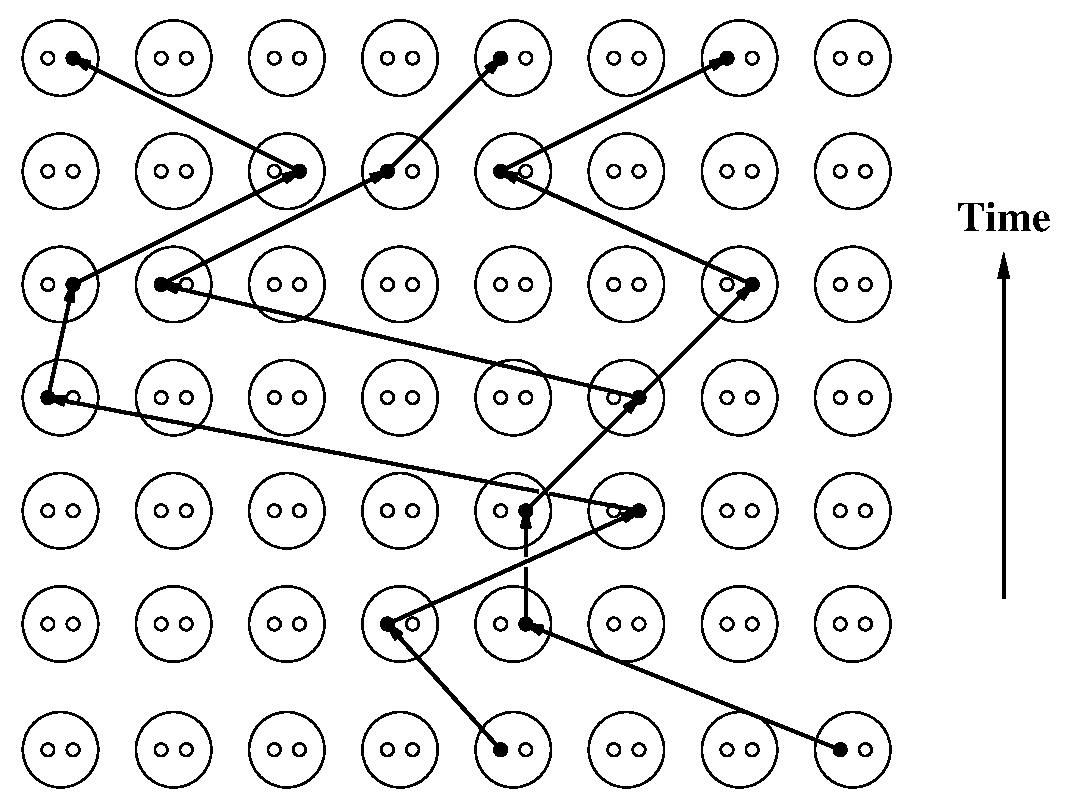
\includegraphics[width=5in]{fig1.idraw}}


\end{document}

Bishop, M. J. and A. E. Friday.  1985.  Evolutionary trees from nucleic acid and
protein sequences.  Proc. Roy. Soc. London  B 226: 271-302

Chakraborty, R.  1977.  Estimation of time of divergence from phylogenetic 
studies.  
.ul
Canad. J. Gen. Cytol.  
19: 217-223

Churchill, G.A.  1989.  Stochastic models for heterogeneous DNA sequences.
{\it Bulletin of Mathematical Biology}  {\bf 51:}  79-94.

{\sc Olsen, G. J.}  1987.  Earliest phylogenetic branchings: comparing rRNA-based
evolutionary trees inferred with various techniques.  Cold Spring Harb.
Symp. Quant. Biol. {\bf 52:}825-837.




